%
% PKUMpLtX --- A LaTeX document class for 'Modern Physics Laboratory' in PKU based on `revtex4-2`
%
% Please read `README.md' and the template file before using
% 需要确保 font 选项指定的字体已安装! 具体参见 `README.md' 的说明.
\documentclass[font=fandol]{mpltx}

% 以下至 \begin{document} 都仅是本文件为了方便额外定义的命令, 写报告时不需要.
\hypersetup{colorlinks=true}% 超链接带颜色
\usepackage{xcolor}
\usepackage{tcolorbox}

\newtcbox{\buttombox}[1][red]
  {on line, arc = 3pt, outer arc = 3pt,
    colback = #1!10!white, colframe = #1!50!black,
    boxsep = 0pt, left = 2pt, right = 2pt, top = 1pt, bottom = 1pt,
    boxrule = 1pt}

\newcommand{\note}[1]{{\color{gray}#1}}
\NewDocumentCommand{\pkg}{s o m}{%
    \IfBooleanF{#1}{%
        \IfNoValueTF{#2}%
            {\href{https://www.ctan.org/pkg/#3}}%
            {\href{https://www.ctan.org/pkg/#2}}%
    }%
    {\textsf{#3}}%
}
\newcommand*\cs[1]{\texttt{\textbackslash #1}}
\newcommand*\env[1]{\textit{\texttt{#1}}}
\newcommand*\code[1]{\texttt{#1}}
\newcommand*\file[1]{\textbf{\texttt{#1}}}
\makeatletter
\newcommand\releasedate{%
    \href{https://github.com/CastleStar14654/PKUMpLtX/releases/tag/\mpltx@fileversion}%
        {\mpltx@filedate, \mpltx@fileversion}}
\makeatother
% 以上是本文件为了方便额外定义的命令, 写报告时不需要.

\begin{document}

\title{体效应振荡器的工作特性和波导管的工作状态} % 切合报告内容, 简短明确, 可以不同于讲义
\author{罗俊熙} % 这里 \emailphone 一定要紧跟在 \author 后方
\emailphone{see.looooo@stu.pku.edu.cn}{(86)13611162432}
% 如果改用 \email 则仅需要邮箱参数
\affiliation{北京大学物理学院\quad 学号: 2000012508}
% % 可以使用 \zhdate 自动生成中文日期, 如
% \date{\zhdate{2020/12/1}}
% % 也可使用 babel 的 \localedate, 如
% \date{\localedate{2020}{12}{1}}
% % 两者均会输出 `2020 年 12 月 1 日'
% 下面的 \date 的参数是为了自动输出正确版本号, 正式报告请替换为上面的两种 \date 之一
\date{\releasedate}
\begin{abstract}
	此部分为摘要.
	200--300字, 说明用什么方法做了什么事, 由此得到什么结果和结论, 有何意义.
	摘要中不用缩略词, 不用第一人称.
	\note{本文档为对 \href{https://github.com/CastleStar14654/PKUMpLtX}{\pkg*{PKUMpLtX}} 的使用示例, 灰色部分为额外针对 \LaTeX{} 模板使用的说明或是一些能提升输出效果的琐碎细节.
		也请注意查看源文档 \file{template.tex} 中的注释.}
\end{abstract}
\keywords{关键词1, 关键词2, 共2--4个}

\maketitle

\section{引言}
微波是一種波長很短,頻率很高的電磁波,其性質讓其很好地應用在國防、通訊和農業生產上,為了了解微波的產生和傳輸特性,掌握有關微波的基本參量,如功率、頻率、電壓和駐波比等的測量原理和方法是必不可少的。
微波通常由一些特殊的電子管如速調管和磁控管等產生,而實驗中常使用體效應振蕩器和雪崩振蕩器等來產生微波。這次實驗就使用了體效應振蕩器產生的微波源。
微波能在波導管中傳播,分為三種狀態:匹配狀態、駐波狀態和混波狀態,而其在波導中傳播的相速度大於光速,可以通過測量頻率和波導波長的方法來確定相速度、群速和和光速。
本次實驗主要是了解體效應振蕩器的一些性質,並掌握微波三種基本參量的測量方法,確定波導波長和波導管中的傳播速度。

\section{理论}\label{sec:theory}
\subsection{體效應振蕩器}
體效應振蕩器主要通過Gunn效應,在n型的砷化錠單晶上產生很高的電流振蕩,然後輻射出微波。這個效應的成因是因為這種材料具有負的微分迁移率的區域,令內部產生“高場疇”,當高場疇傳播到導體邊界時,就會產生電流脈衝,進而轉化為微波。
這種脈衝是週期性的,其頻率為:
$$f=\frac{1}{T_D}=\frac{v_d}{f}$$
式中,$T_D$是疇的渡越時間,而$L$為樣品的長度,$v_d$為畴的運動速度。
\subsection{體效應振蕩器的工作特性}
將體效應二極管放在高$Q$的諧振腔中,構成電路,就能產微波振湯,而本次實驗使用的固態源則是使用機械調諧的方式,產生特定頻率的微波。機器內部具有一個非接觸活塞,可以改變諧振腔的有效長度,改變振蕩頻率,活塞移入腔內越多,電容減少,工作頻率提升。因為每個體效應二極管的摻雜、缺陷或位錯等都不一樣,因此其工作電壓、頻率等關系都不一樣。
\subsection{波導管中波的傳播特性}
波導管中能通過特定波長的電磁波,由於麥克斯韋方程式的限制,電磁場在其內部只能以特定的模式傳播,這次實驗的方形波導管,就只能通過$\rm{TE_1}$的模式,其特色是在導管中形成垂直波導寛壁的電場,而且傳播的波導波長和自由空間並不一樣。滿足:
$$c=\lambda f, \quad v_g=\lambda_gf$$
其中$c$為光速,$v_g$為相速度。而理論表明,光在其內的相速度是大於光速的。因此我們可以通過測定波導波長$\lambda_g$和頻率$f$來找出光速$c$。
\subsection{駐波測量}
我們可以通過駐波測量線來進行駐波比和波導波長的測量,將系統調節至匹配的狀態,而駐波比則是如下定義的
$$\rho\frac{|E_{\max}|}{|E_{\min}|}$$
其中$E$為駐波線測得的場強。調節的方法則是通過單螺螺調配器和駐波測量線的交互調節,來形成不同的駐波比,,駐波比反射率有着以下關係:
$$\Gamma_0=\frac{\rho -1}{\rho+1}$$
這次實驗的後半部分,需要在駐波的狀態下進行。
\subsection{檢波特性曲線和檢波律}
在測量駐波比時,檢波晶體會有輔出信號測出,晶體的檢波電流$I$和傳輸線探針周圍的電場$E$滿足:
$$I=k_1E^n$$
其中$k_1$和$n$都是一些常數,一般地$n$都很接近$2$,稱為平方律檢波。進行測量時,會先將測量線終端短路,駐波振幅與終端距離滿足的關系為:
$$|E|=k_2|\sin{\frac{2\pi l}{\lambda_g}}|$$
我們可以通過檢波電流關於$l$的曲線$I(l)$和$E$來求得常數$n$進而得到晶體的檢波律,一般地,我們可以用下列關系式定出$n$:
$$n=\frac{-0.3010}{\log_{10}{\cos\frac{{\pi\Delta l}}{\lambda_g}}}$$
其中$\Delta l$為駐波曲線上$I=I_m/2$兩點距離。

\section{实验装置}
本次實驗使用的微波信號由DH1121A型3cm固態信號源提供,而主要元件有隔離器、衰減器、吸引式頻率計、駐波測量線和單螺調配器。如图\autoref{fig:1}搭建線路,其中A和B都是電流錶,用以示波作用。
\begin{figure}
	\centering
	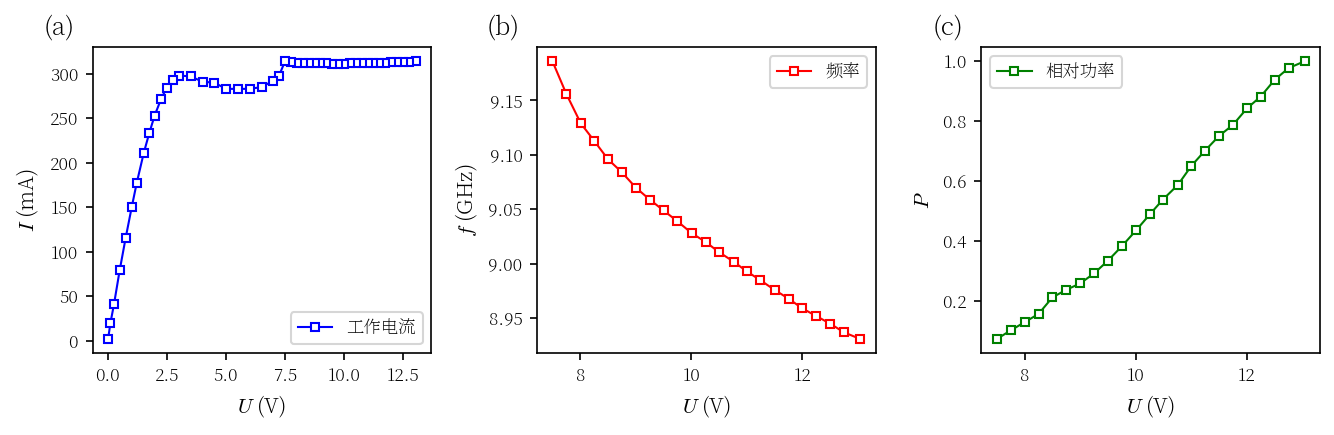
\includegraphics[width=0.85\linewidth]{fig/1.png}
	\caption{\footnote{吳思誠、荀坤.近代物理實驗(第四版).北京:高等教育出版社}實驗線路圖}
	\label{fig:1}
\end{figure}

\section{實驗內容}
\begin{enumerate}
	\item 测量体效应振荡器的工作电压与工作电流、输出功率及频率的特性曲线;
	\item 测量振荡频率和輸出功率的关系曲线;
	\item 調節和测量小驻波比和中驻波比的線路,並計算其反射率$\Gamma_0$;
	\item 测量波导波长、光速、相速度和群速度;
	\item 測量驻波曲线和計算出檢波律常數$n$。
\end{enumerate}

\section{實驗過程、结果及讨论}
\subsection{观测体效应振荡器的工作特性}
将信号源置于\buttombox[blue]{等幅}状态,调节\buttombox[blue]{频率},使其至$\qty{9.000}{\GHz}$,预热$\qty{30}{\minute}$。
\par
按下\buttombox[blue]{教学},通过\buttombox[blue]{电压}按钮,在$0\sim\qty{13.0}{\V}$连续改变工作电压,得到频率计和光点检流计B,测得微波频率和相对功率(注要调节短路活塞和单螺调配器),使检波接头输出最大。实验结果如下图所示:

图在这。

\subsection{改变谐振腔的有效长度,测量振频率和輸出功率的关系曲线}
提起\buttombox[blue]{教学},使其工作在标准电压$\qty{12.0}{\V}$,此时的工作电流约为$\qty{250}{\mA}$,转动\buttombox[blue]{频率},改变谐振腔尺寸,从而改变其微波频率,然后用频率计做频率测量,得到下图:

图在这

\subsection{练习测量小驻波比和中驻波比}
在\buttombox[blue]{等幅}状态下,使频率显示为$\qty{9.000}{\GHz}$,电压为$\qty{12.0}{\V}$,调整好驻波测量线,利用单螺调配器改变测量线的终端状态,调节到匹配状态,测量小驻波比,如下表

表在这

可以求出,这是的小驻波比为$\rho=$

\subsection{测量波导波长}
调节单螺调配器,使驻波测量线终端接近全反射(即$\rho$值较大),利用平均值法测量极小点两侧的等强点$x_1',x_1''$,用平均值的方式求得$x'_{\min}=\frac{1}{2}(x_1'+x_1'')$,这里则用三个波节作线性拟合:$x_n=\lambda_g\times n + c$,得到下表

表在这

可以得到$\lambda_g= 1$

再利用自由空间波长关系:$\lambda=\frac{\lambda_g}{\sqrt{1+(\frac{\lambda_g}{2a})^2}}$,其中波导管寛边为$a=\qty{22.86}{\mm}$,而频率测得为$f=$得到光速为$c=\lambda\times f$,相速度$v_g=\lambda_g\times f$,群速度$u=\frac{c^2}{v_g}=\frac{\lambda^2f}{\lambda_g}$

\subsection{驻波曲线}
调节单螺调配器,使驻波测量线终端完全短路,(即$\rho$值非常大),在两个波节间,测出检波电流$I$和线上电场强$|E|$,并画出$I-|E|$的图\ref{1},如下所示:

图在这

可以看出在$I=\frac{1}{2}I_m$的时侯,终端距离分别为$l_1=1,l_2=2$,利用公式$n=\frac{-0.3010}{\lg{\cos{\frac{\pi\Delta l}{\lambda_g}}}}$,得到检波律$n$为:
$$n=1.0$$

此部分是实验报告的主体, 应占报告篇幅的一半以上.
\note{依自己意愿, 结果与分析部分可以分多个小节, 甚至可以将实验结果和对结果的分析讨论拆分为两节.}

实验结果应尽量以图表的形式给出. 每一个图表都应该是完整的, 即阅读图表时可以不必依赖正文.
以图表为中心叙述实验结果和讨论.

\subsection{表格}\label{ssec:table}
\subsubsection{表格}\label{sssec:table}


表是被一系列横线隔开的有序排列的数据, 报告格式要求最上和最下两条横线为双横线.
\note{此双横线格式可以通过 \env{ruledtabular} 环境和 \cs{colrule} 命令实现.}
例表为\autoref{tab:table_eg}.

\begin{table}
	\caption{表格示例%
		\footnote{表格标题要简明扼要; 注意使用 \pkg[revtex]{revtex4-2} 提供的 \env{ruledtabular} 环境生成首尾双横线的表格.
			表格中的脚注会自动加在表尾.
			为方便, 提供了 \cs{mc} 作为 \cs{multicolumn} 的简写.
			\href{https://www.tablesgenerator.com}{Tables Generator 网站}可以方便地生成 \LaTeX 表格.}}
	\label{tab:table_eg}
	\begin{ruledtabular}% ruledtabular 环境自动生成首尾双横线, 并调整宽度至占满全行
		\begin{tabular}{cd{4.2}lr}
			% d{a.b} 能使该列中的数据按小数点对齐, 前方留 a 个字符, 后方留 b 个字符
			% 已将 multicolumn 简写为 mc
			居中  & \mc{1}{c}{数值                 %
				\footnote{``数值'' 列使用了 \code{d} 列格式来按小数点位置对齐. 记得将 \code{d} 列的列标题单独设为居中.}
			}     & 靠左           & 靠右          \\
			\colrule% 中间横线
			a     & 0.12           & a     & a     \\
			bbb   & -100           & bbb   & bbb   \\
			ccccc & 50.8           & ccccc & ccccc
		\end{tabular}
	\end{ruledtabular}
\end{table}

从\autoref{tab:table_eg} 可以看出, 对表中各项的注释应作为表的一部分放在表后, 而不是页脚或文尾.
\note{在表格中使用 \cs{footnote} 命令时 \LaTeX 会自动将注释放在表尾.
	但正文中的注释按照 AIP 的要求 (以及 \pkg[revtex]{revtex4-2} 的实现) 是会和各引用项共同编号并作为参考文献列表的一部分的.
	因此, 只要你在正文使用了 \cs{footnote}, 即使你没有引用任何文献 (这一般不太可能), 也需要用 B\textsc{ib}\TeX 处理.
	这里是一个尾注的例子 \footnote{这里是一个尾注的例子}.}

当原始数据和处理过的数据常需要出现在同一表中时, 用软件来处理会非常方便.
但出现在实验报告中的表应具有上面给出的例子的格式.

\subsection{数据图}

\textbf{每个图应尽量让读者不看正文就能基本理解图的含意.}
应包含: 图名、轴名、轴、刻度、标尺、数据点、曲线、图例、标注和图注等部分.
最常用的作图软件有 Origin 或 MATLAB.
学习使用基本的数据处理和作图工具软件也是课程的基本内容.
课程也鼓励大家使用 Python 语言编程作图.
逐点测量得到的函数关系要同时用表格和图给出.
\note{数据点过多可以将数据放到附录.
	这里 ``逐点测量得到的函数关系'' 还是要自己把握一下, 像那种几千个数据点的能谱当然就没必要放原始数据表了.}
\textbf{需要作比较的多条曲线要画在同一图上.}
为避免读者在图表和正文间反复跳跃阅读, 正文叙述应紧邻图表, 正文中也要对图表作必要的说明.

\begin{figure}
	\centering
	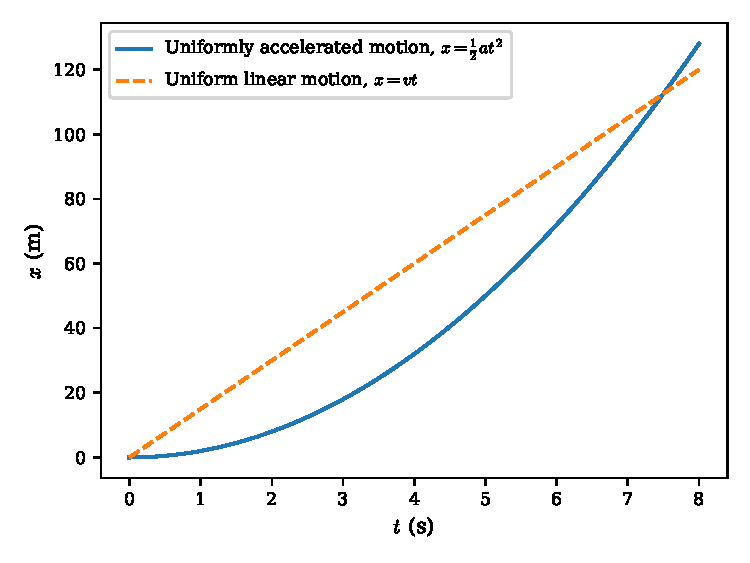
\includegraphics[width=0.8\textwidth]{fig/figsample.pdf}
	\caption{这是数据图的例子.
		\note{在图的 \cs{caption} 中应简要说明图中表达的内容, 并对各种符号、线型、颜色的意义做出说明.
			如果有多格数据图, 应清晰地分别做出解释说明.
			图中的关键性文字 (比如轴名和图例) 的大小最好能和说明文字中的文字大小相当.
			关于坐标轴名和单位的标法, 可以参看\href{https://journals.aps.org/authors/axis-labels-and-scales-on-graphs-h18}{美国物理学会的说明}.
			本图是用脚本 \file{figgen.py} 生成的}}
	\label{fig:data}
\end{figure}

\autoref{fig:data} 是一张例图.

\subsection{对分析的要求}

对于预料之外的实验结果, 必须首先小心证明其可靠性.
读者只有在相信你的实验结果时才愿意花时间看你的分析.

\textbf{必须用文字归纳整理出正式的实验结果或结论.}
可信的实验结果是课程报告最重要的内容.
作为一个实验物理工作者, 分析解释出错并不丢脸, 实验结果不被采信则是致命的.
教学实验的结论往往是预先知道的.
所以, 教师更关心的是你的说理过程.
一般说来, 单由课内实验的结果不足以能得到明确的结论.
此时, 你可以引用他人的研究结果来帮助帮助自己的论证, 但必须注明出处.
确实不能得到明确结论时, 可以给出几种可能结论并指出可以再做哪些实验来帮助作进一步的判断.
总之, 分析讨论部分要做到: 论据要valid, 论证要reasonable, 结论要convincing.

\section{结论}
\textbf{文字写一段.}
首先要给出实验结果, 然后再给出由实验结果分析得到的结果和结论.
此部分给出的内容要比摘要中的全面, 用词要更准确.

\begin{acknowledgments}
	感谢对实验和报告有具体重要帮助的, 又没被列为作者的人.
	\note{撰写致谢时请使用 \env{acknowledgments} 环境.}
\end{acknowledgments}

% bibliography 的参数是你的 *.bib 文件去掉后缀名后的部分
\bibliography{bibli}

\clearpage % 附录前另起一页
\appendix % 附录开始
\section{思考题}\label{app:exercise}
\subsection{可以把每道思考题的题目分别作为小标题}
然后书写解答.

\section{近代物理实验报告写作要求}

物理实验的结果最终需要以论文或报告的形式向同行或公众报道.
外界也主要基于这些论文或报告来评价一个实验物理工作者.
所以, 课程实验报告的撰写是北大 ``近代物理实验'' 课的一个重要内容和主要的评分依据.

北大近代物理实验课要求按研究论文的形式来撰写课程实验报告.
和任何期刊一样, 近代物理实验课对学生提交的课程实验报告也有内容和格式上的要求.
学生应依照课程提供的课程实验报告模板来撰写自己的实验报告.

课程提供的课程实验报告模板综合了 American Institute of Physics (AIP) 期刊和中国《物理学报》对稿件格式的要求.

本实验报告模板各部分的文字给出了相应节写作时应注意的问题.

\subsection*{报告写作的一般事项}

\begin{enumerate}
	\item 课程实验报告应假定读者既不是已知全部实验细节的指导教师, 也不是缺少专业知识的公众, 而是同领域的实验研究者, 或审稿人.
	      不能要求读者要在读过课程讲义后才能读懂课程实验报告.
	\item 文本和物理量单位用正体, 物理变量符号用斜体, 矢量矩阵符号用黑斜体.
	      \note{(\pkg{physics} 宏包提供了大量的方便的物理中常用符号的排版工具, 请参考其文档使用)}
	\item 使用国际标准的缩略词, 符号和法定计量单位时应全文一致, 正文中的缩略
	      词在\textbf{首次出现时写出全称}, 后附缩略词, 并用括号括起; 之后直接用缩略词, 不
	      再写全称, 如 American Institute of Physics (AIP).
	\item 全文标点符号除 ``顿号'' 外, 其他用英文半角标点符号.
	      \note{(推荐的格式中, 英文单词和数字应与汉字之间插入一个空格;
		      半角标点符号应如英文一般, 在逗号, 句号, 分号等后方插入一个空格;
		      在引号, 括号外侧各插入一个空格;
		      连续出现的标点符号之间的多余空格则应删除.
		      但是, \pkg{xeCJK} 宏包基本上自动为你在最终的 PDF 文稿中完成了这些事情.
		      此外, 如果你觉得半角符号配中文太丑, 请参见 \file{README.md} 中介绍的标点选项)}
	\item 公式、图和表要分别用阿拉伯数字编列序号. \note{(这点 \LaTeX 可以为你代劳)}
	      公式和图表要达到可发表的质量.
	\item 凡不是自己独立思考得到的内容都应该引参考文献.
	      不能大段引用同一参考文献.
	      对复杂问题, 应该优先考虑引用参考文献得到结果.
	      对简单一些的问题才鼓励独立思考.
	      只能引用正式出版物, 不能引用他人实验报告.
	\item 模板中的未尽事项可以参考 AIP Style Manual 4th-edition (可从课程网站下载).
	      \note{(也可参考 \pkg[revtex]{revtex4-2} 的文档)}
	\item 较长的推导和说明可以作为附件提交, 不占用报告篇幅.
	\item 思考题不是报告的组成部分.
	      应另起一页附在报告的最后. \note{(比如作为附录)}
\end{enumerate}

\section{对 \LaTeX{} 中标点输入的额外说明}
\LaTeX 中对 dash 有所区分,
\begin{center}
	\begin{tabular}{c@{\quad}c@{\ $\rightarrow$\ }c}
		连字符 hyphen      & \verb|co-operate|   & co-operate   \\
		连接号 en-dash     & \verb|14--19|       & 14--19       \\
		英文破折号 em-dash & \verb|Yes---or no?| & Yes---or no? \\
		减号               & \verb|$-1$|         & $-1$         \\
	\end{tabular}
\end{center}
中文破折号 (——) 就按一般习惯的用输入法输入即可.
\note{其实中文破折号就是两个连着的 em-dash, 但两种输入方式使他们输出字体不同.}

\LaTeX 中半角引号使用如下映射进行输入.
左引号的符号为 \textsf{Esc} 键下方的锐音符.
\begin{center}
	\begin{tabular}{c@{\quad}c@{\ $\rightarrow$\ }c@{\quad}c@{\ $\rightarrow$\ }c}
		单引号           & \verb|`|     & `     & \verb|'|     & '     \\
		双引号           & \verb|``|    & ``    & \verb|''|    & ''    \\
		美式连续嵌套引号 & \verb|```|   & ```   & \verb|'{}''| & '{}'' \\
		英式连续嵌套引号 & \verb|`{}``| & `{}`` & \verb|'''|   & '''   \\
	\end{tabular}
\end{center}
注意其中 \code{\{\}} 起到的分组作用.

此外, 如果想使用全角符号同时想使用实心点格式的句号, 可以使用 \code{quanjiao} 选项.
源文档中的 ``。'' 会被自动替换成 ``.''.
这时, 也就可以风格统一地直接使用中文输入法给出的引号 ``“”‘’'' 而不用管前面提到的映射了.
具体请参见 \file{README.md} 中介绍的标点选项.

\note{其实“和``以及”和''分别是同一个 Unicode 字符, 只是被分配了不同的字体.}

\section{DIY 字体效果测试}

\newcommand{\testword}{报告}
\newcommand{\andbold}{\testword{}\textbf{\testword{}}}
\newcommand{\testline}{\testword{}\emph{\andbold{}}\andbold{}}

下面分别展示衬线, 无衬线和等宽中文字体效果, 便于检查基线高度等问题.
\begin{center}
	\textrm{\testline}\\
	\textsf{\testline}\\
	\texttt{\testline}
\end{center}

\end{document}
